% Beamer drop-in for JRC C4 deck slide-26 position.
% Compile:  xelatex jrc_section.tex   (run twice for page-number resolution)
\documentclass[aspectratio=169,11pt]{beamer}
\usepackage{fontspec}
\setsansfont{Helvetica Neue}[Scale=0.95]
\setmonofont{Menlo}[Scale=0.85]
\usepackage{xcolor}
\usepackage{graphicx}
\usepackage{tcolorbox}
\tcbuselibrary{skins}
\usepackage{tikz}

% JRC palette: title blue, neutral grey body, persona accents.
\definecolor{jrcblue}{HTML}{3B3B8C}
\definecolor{l1grey}{HTML}{7F7F7F}
\definecolor{l2amber}{HTML}{D97706}
\definecolor{l3orange}{HTML}{EA580C}
\definecolor{cardbg}{HTML}{FAFAFA}
\definecolor{cardborder}{HTML}{CCCCCC}

% Theme: plain background, no navigation, JRC-blue titles.
\usetheme{default}
\setbeamertemplate{navigation symbols}{}
\setbeamercolor{frametitle}{fg=jrcblue,bg=white}
\setbeamercolor{normal text}{fg=black,bg=white}
\setbeamerfont{frametitle}{size=\Large,series=\mdseries}
\setbeamerfont{itemize/enumerate body}{size=\normalsize}
\setbeamertemplate{itemize item}{\color{jrcblue}\textbullet}
\setbeamertemplate{itemize subitem}{\color{jrcblue}\textendash}
\setbeamertemplate{footline}{%
  \hfill\raisebox{6pt}{\tiny\color{gray}\insertframenumber\hspace{6mm}}%
}
\setbeamertemplate{frametitle}{%
  \vspace{6pt}\hspace{4pt}\insertframetitle\par\vspace{-4pt}%
}

% Big-headline number macro (sits inside a columns environment).
\newcommand{\bignum}[3]{%
  \centering
  {\fontsize{40pt}{44pt}\selectfont\textbf{\textcolor{#1}{#2}}}\par
  \vspace{4pt}{\small\textbf{\textcolor{#1}{#3}}}\par
}

% Persona-card macro (sits inside a columns environment).
\newcommand{\personacard}[4]{%
  \begin{tcolorbox}[
    colback=cardbg, colframe=#1, boxrule=1.2pt, arc=3pt,
    left=6pt, right=6pt, top=4pt, bottom=4pt,
    valign=top, height=4.6cm,
  ]
    \textbf{\textcolor{#1}{#2}}\\[2pt]
    \small #3\\[6pt]
    \scriptsize\textcolor{gray!50!black}{#4}
  \end{tcolorbox}%
}

\begin{document}

% ----- Slide 1 -----
\begin{frame}{Practical Use: Writing Code \& Data Viz (4 min)}
  \begin{itemize}
    \item \textbf{Speaker:} Dermot
    \item \textbf{Question:} Q4 --- How can we use AI to write simple scripts and
          data visualisation code? What tools are best?
    \item \textbf{What I'll show:} the \emph{same} AI agent (Claude Code, Opus 4.7)
          on the \emph{same} forecasting task, with three different ways of asking.
          The error fell by a factor of three.
  \end{itemize}
  \vspace{8pt}
  \begin{columns}[t,onlytextwidth]
    \begin{column}{0.32\textwidth}\bignum{l1grey}{10.76\%}{L1 --- beginner prompt}\end{column}
    \begin{column}{0.32\textwidth}\bignum{l2amber}{5.52\%}{L2 --- average user}\end{column}
    \begin{column}{0.32\textwidth}\bignum{l3orange}{3.43\%}{L3 --- research-grade prompt}\end{column}
  \end{columns}
  \vspace{8pt}
  \begin{center}\small
    MAPE on a held-out 168-hour forecast of German hourly electricity load
    (Open Power System Data).
  \end{center}
\end{frame}

% ----- Slide 2 -----
\begin{frame}{Three users, three prompts, three workspaces}
  \begin{columns}[t,onlytextwidth]
    \begin{column}{0.32\textwidth}
      \personacard{l1grey}{L1 --- beginner}{One sentence. No project setup.}{%
        Prompt: \textbf{10 words}\\
        AGENTS.md: \emph{none}\\
        Output: three baselines, no validation}
    \end{column}
    \begin{column}{0.32\textwidth}
      \personacard{l2amber}{L2 --- average user}{Names the data file, the horizon, the libraries.}{%
        Prompt: \textbf{46 words}\\
        AGENTS.md: 7 lines\\
        Output: one model, no intervals}
    \end{column}
    \begin{column}{0.32\textwidth}
      \personacard{l3orange}{L3 --- research-grade}{Structured prompt (TASK / BACKGROUND / DO NOT). Detailed workspace context.}{%
        Prompt: \textbf{1{,}673 words}\\
        AGENTS.md: 113 lines\\
        Output: 6-model bake-off + calibrated intervals + methods writeup}
    \end{column}
  \end{columns}
  \vspace{6pt}
  \begin{itemize}\small
    \item The headline gap is not about typing more --- it's about specifying every
      dimension that matters: \textbf{task, data, models, splits, metric, format,
      things-not-to-do.}
  \end{itemize}
\end{frame}

% ----- Slide 3 -----
\begin{frame}{Where each model fails --- the diagnostic L3 forced}
  \begin{center}
    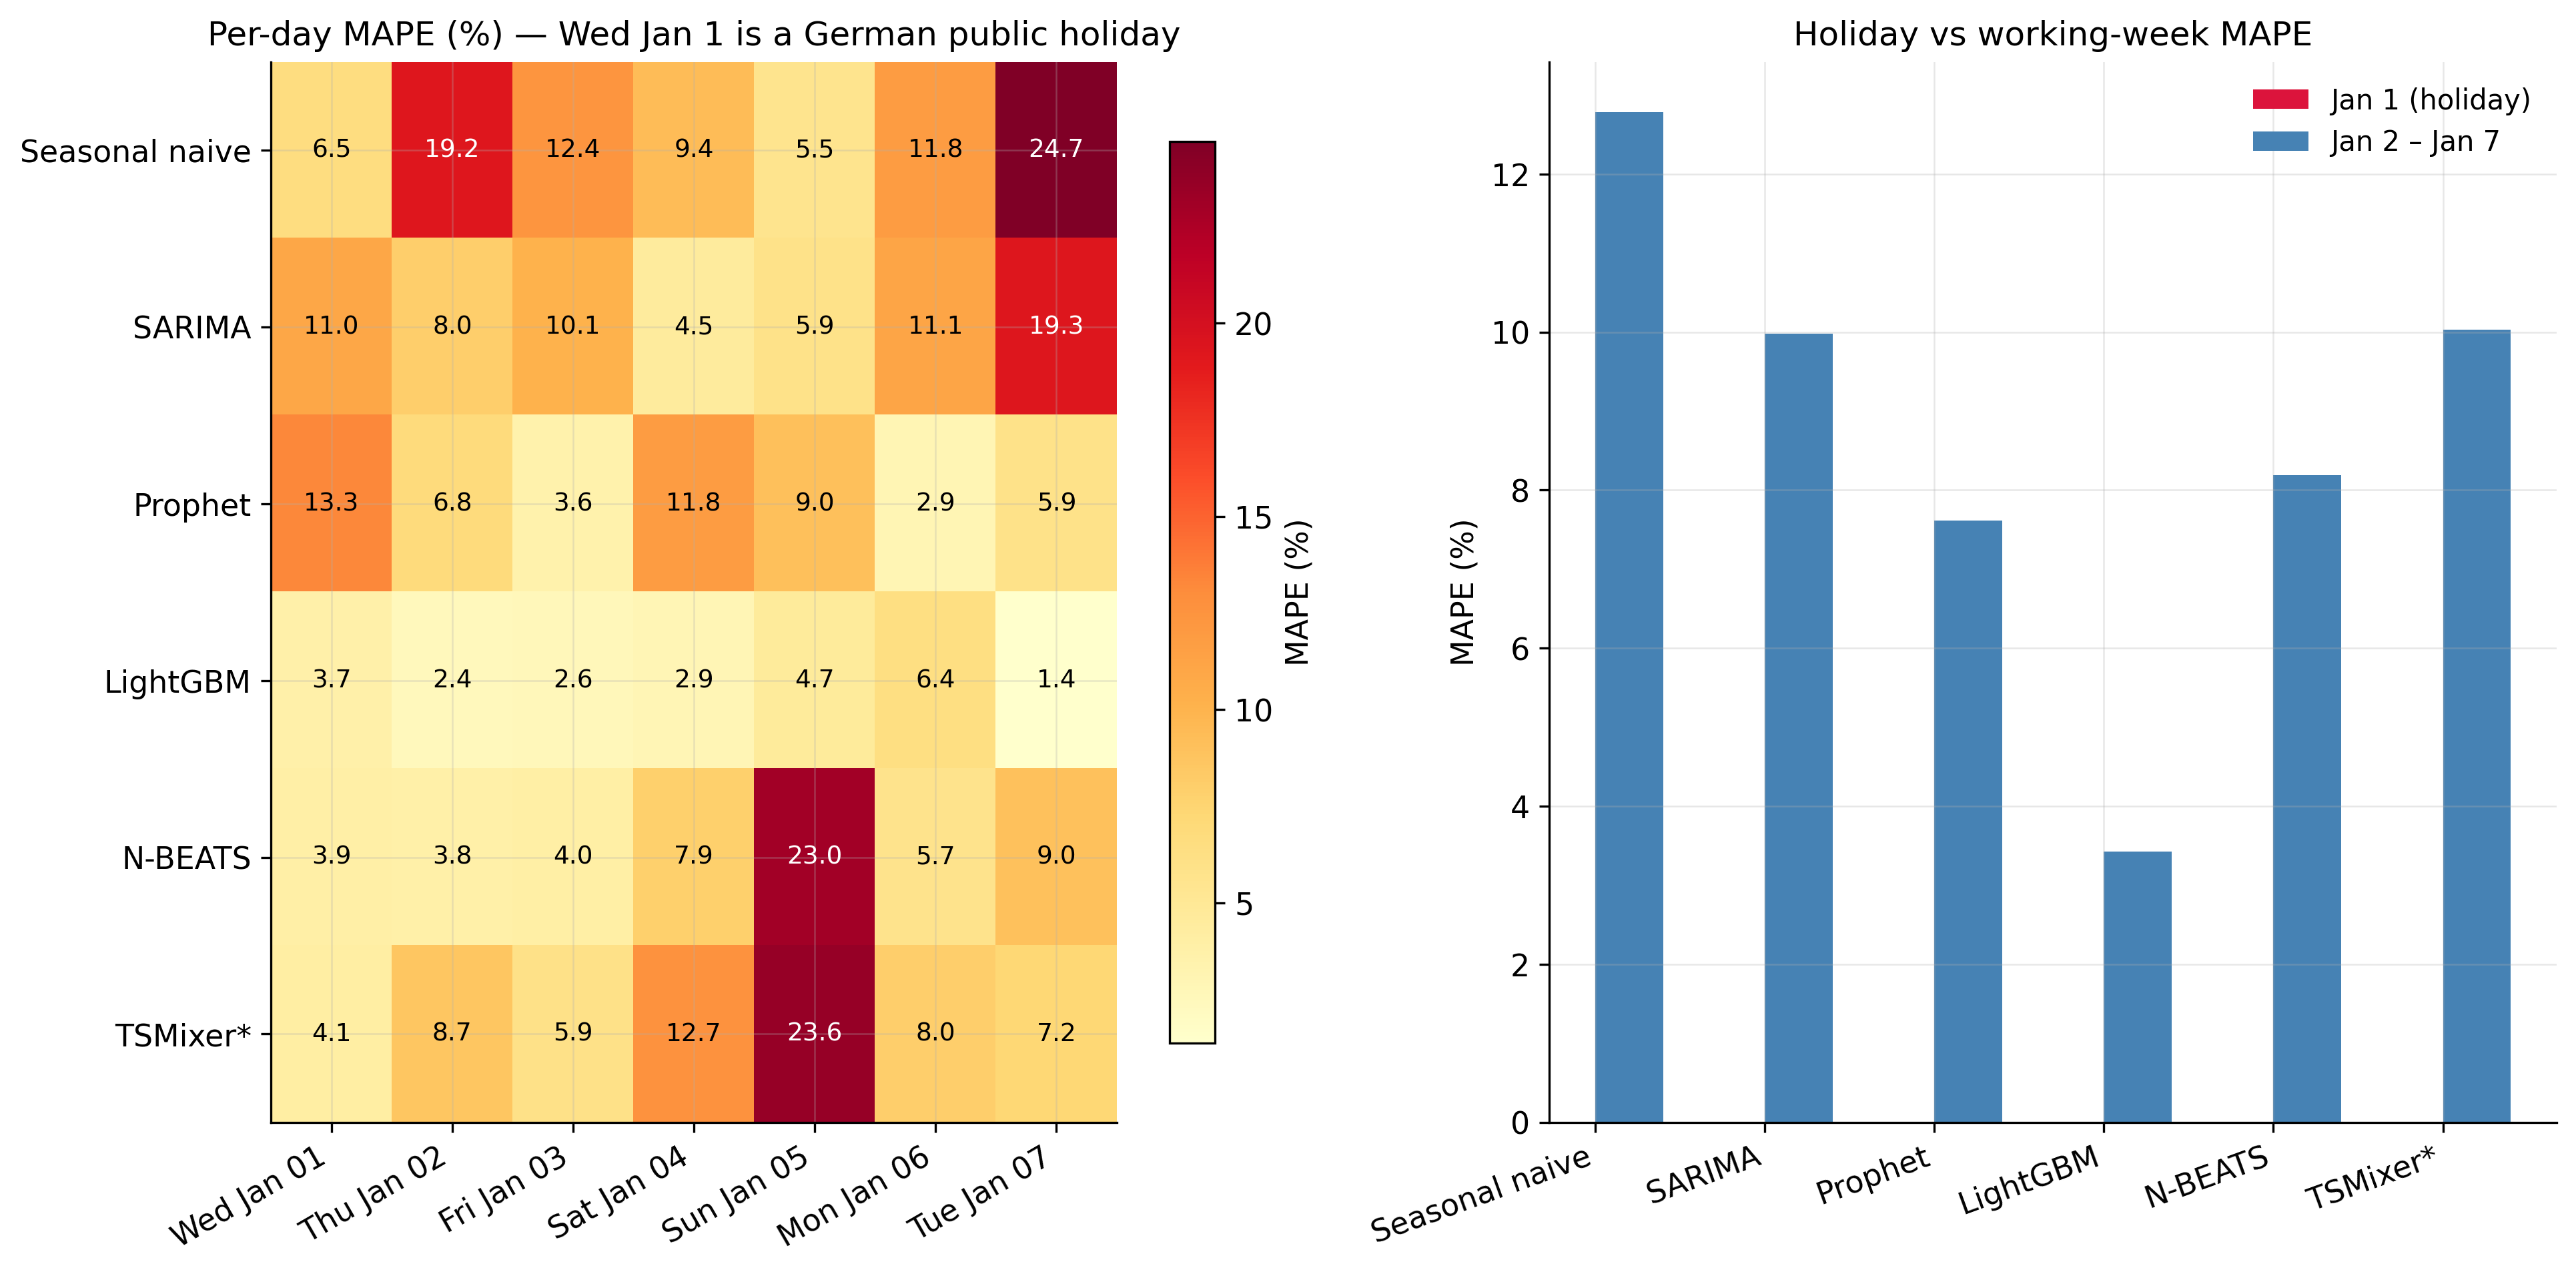
\includegraphics[height=0.62\textheight]{../runs/L3/figures/04_per_day_mape.png}
  \end{center}
  \begin{itemize}\small
    \item Only \textbf{LightGBM} stays uniformly low across the week; 80\%/95\% intervals are
      calibrated at \textbf{79.8\%} / \textbf{92.9\%}. This per-day breakdown does not exist
      for L1 or L2 --- they were never asked for it.
  \end{itemize}
\end{frame}

% ----- Slide 4 -----
\begin{frame}{Four habits that worked here --- and on the next slides}
  \begin{enumerate}
    \item \textbf{Specify what success looks like} --- not just what to build (the metric,
      the format, the splits).
    \item \textbf{Use a DO NOT section} --- the cheapest, highest-leverage block of any prompt.
    \item \textbf{Put standing context in \texttt{AGENTS.md}} --- write it once;
      every future session reads it.
    \item \textbf{Make the AI verify itself} --- a held-out split, intervals or sensitivity
      checks, a written discussion of failure modes.
  \end{enumerate}
  \vspace{4pt}
  \begin{itemize}
    \item Same four habits apply on the next three slides (drafting reports, literature
      reviews, daily co-pilot use).
    \item Repo: \texttt{github.com/DermotOBrien-EC/LLM\_coding\_example\_jrc\_andres}
  \end{itemize}
\end{frame}

\end{document}
